\section{Introduction}
\label{sec:intro}

In Image Segmentation, there are three common types of segmentation tasks: \textit{Semantic Segmentation}, \textit{Instance Segmentation}, and \textit{Panoptic Segmentation}. In Semantic Segmentation, the goal is to classify each pixel in the image into a predefined set of categories (such as "car", "road", "tree", "person", etc.). All pixels that belong to the same category are assigned the same label. Instance Segmentation identifies individual objects within the image and assigns a unique label to each object i.e., it distinguishes between different instances of the same category (such as two cars will be assigned different labels). Panoptic Segmentation combines both semantic and instance segmentation. It aims to provide a complete understanding of the scene by identifying both object instances and background areas. In this work, we focus on the task of Semantic Segmentation.

\begin{figure}[t]
  \centering
  % \fbox{\rule{0pt}{2in} \rule{0.9\linewidth}{0pt}}
   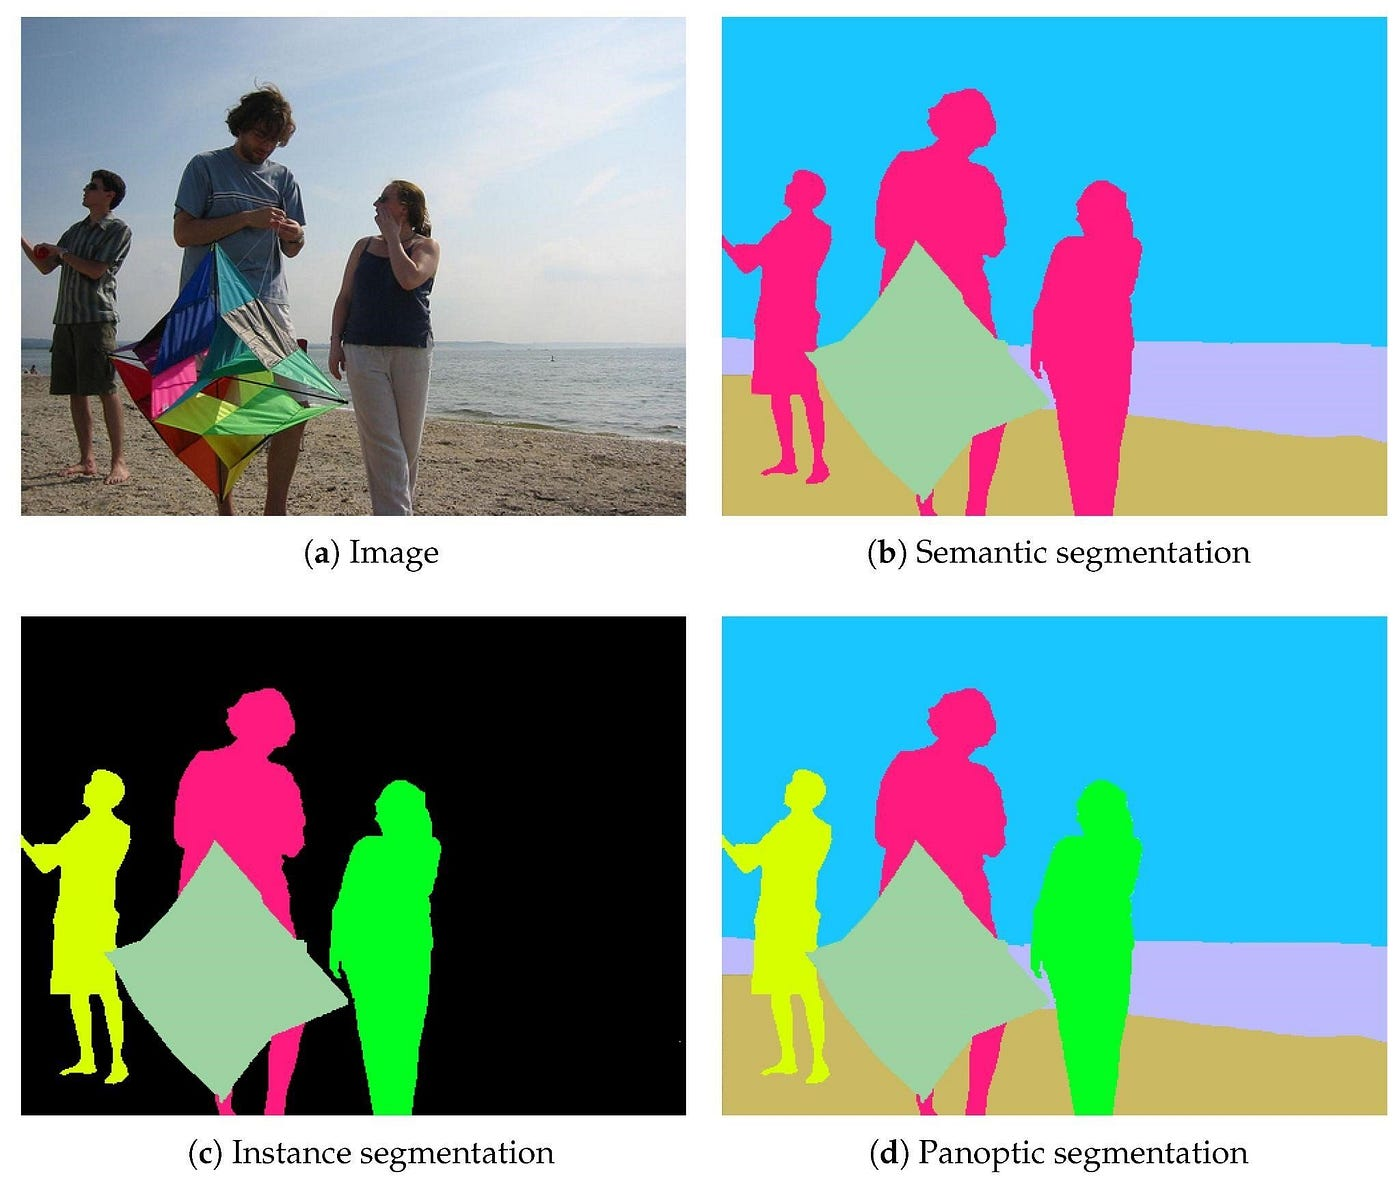
\includegraphics[width=0.8\linewidth]{images/image_seg_example.jpg}

   \caption{An Example showing the three types of segmentation tasks: Semantic Segmentation, Instance Segmentation, and Panoptic Segmentation. From ~\cite{medium_article_1}}.
   \label{fig:onecol}
\end{figure}
